% x 与 y 关系,多对一
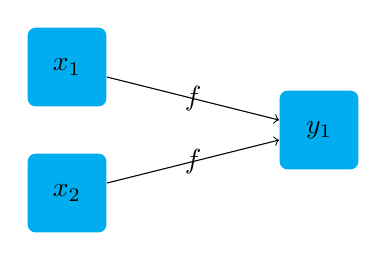
\begin{tikzpicture}[scale=0.8]
  \node [fill=cyan,minimum size=1cm,rounded corners=.1cm]   (x1) at (0,0)    {$x_1$};
  \node [fill=cyan,minimum size=1cm,rounded corners=.1cm]   (x2) at (0,-2)   {$x_2$};
  \node [fill=cyan,minimum size=1cm,rounded corners=.1cm]   (y1) at (4,-1)   {$y_1$};

  \draw [->] (x1) -- (y1) node[midway] {$f$};
  \draw [->] (x2) -- (y1) node[midway] {$f$};
\end{tikzpicture}
